\section{Conclusões e Perspectivas}

    O presente trabalho teve como foco a expansão das possibilidades de recursos da controladora aberta \textit{C5G-Open} através da implementação de um sistema cliente servidor. Os resultados preliminares foram considerados satisfatórios, motivando a continuidade do desenvolvimento dos softwares e do projeto em si. A sub-rede demonstrou garantir a comunicação de forma estável e rápida. A integração dos softwares foi facilitada pela padronização do protocolo TCP/IP, o que ajudou expandir as possibilidades de uso do OpenServer.
    
    A perspectiva futura é usar o OpenSever para dar início ao desenvolvimento de malhas de controle adicionais ao sistema robótico como uma malha de visão computacional. Uma câmera afixada no efetuador do robô filmará uma figura de referência, o software cliente processará a imagem e gerará os comandos de movimentação que serão enviados ao OpenServer, de forma a manter constante a pose (posição e orientação) do manipulador robótico em relação à pose da figura de referência. Dessa maneira, deverá ser adicionada uma câmera à estrutura desenvolvida, conforme pode ser visto na Figura~\ref{pespectiva}, onde (1) representa a câmera; e (2) a figura de referência.
    
    
    \begin{figure}[ht]
        \centering
        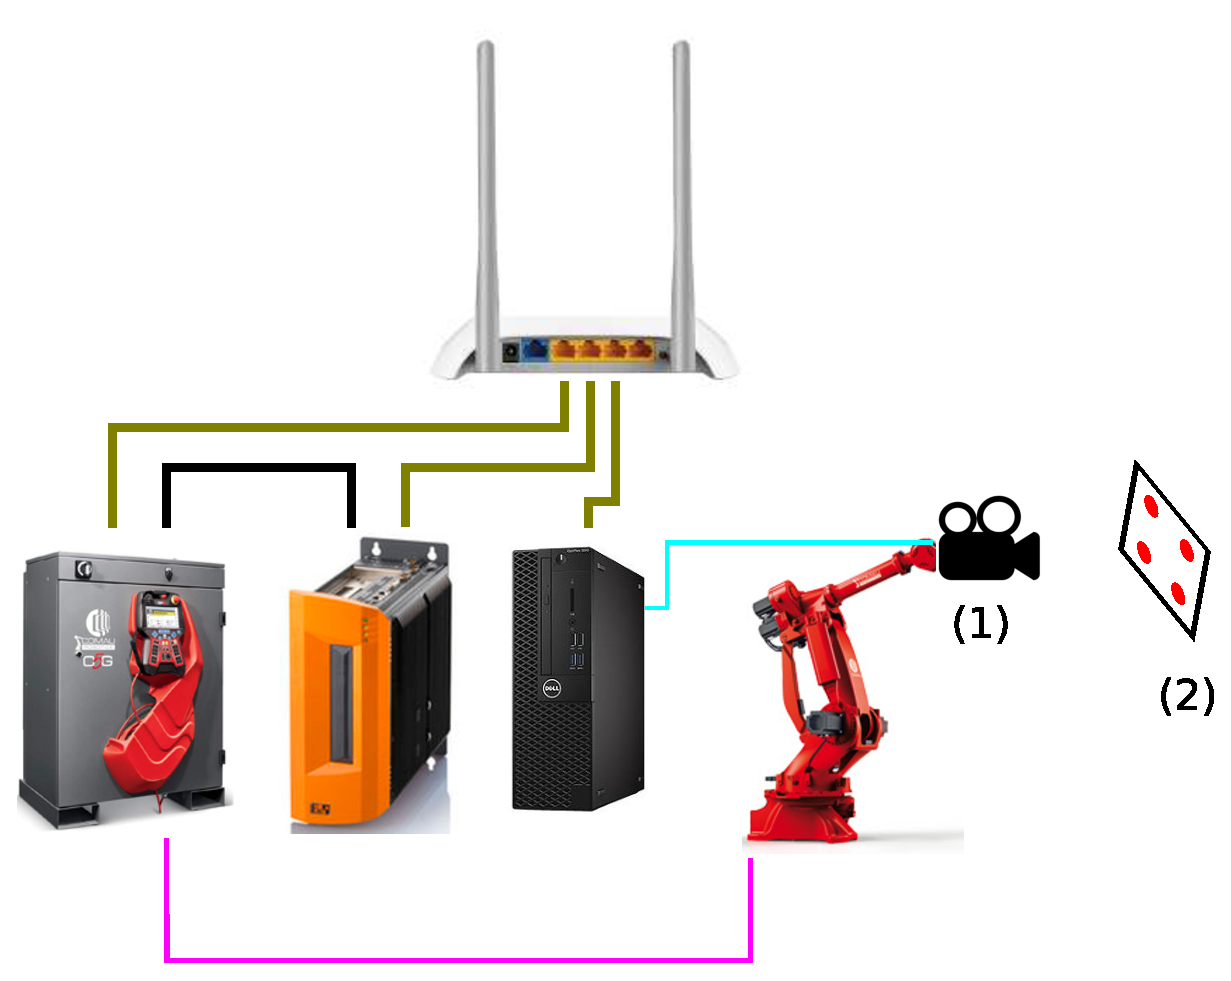
\includegraphics[width=\columnwidth]{imagens/pespectiva.eps}
        \small 
        \centering 
        \caption{Estrutura proposta para utilização do OpenServer}
        
        \label{pespectiva}
    \end{figure}
    
\section{Agradecimentos}
    %E o CEFET-MG ?
    Agradecemos ao CNPq - Conselho Nacional de Desenvolvimento Científico e Tecnológico - pelo apoio financeiro dado a essa pesquisa através da concessão de bolsa do PIBTI - Programa Institucional de Bolsas de Desenvolvimento Tecnológico e Inovação. Agradecemos também a COMAU Robotics pelo suporte técnico e orientações dadas.